\subsection{Interval Analysis Efficiency (Goal 1)}\label{sec:interval_analysis_efficiency}

In this section, we evaluate the efficiency of Nugget's interval analysis.
We define efficiency using two criteria:
(1) \emph{low slowdown}, quantified as the ratio between the time spent on interval analysis and the time required for executing the full workload; and
(2) \emph{flexibility}, meaning the ability to perform the analysis across different host machines.

During interval analysis, we identify all valid intervals and collect two key artifacts: the LLVM IR Basic Block (IRBB) vector and the count-stamp vector (Section~\ref{sec:interval_analysis_executable}).
These outputs are later used to generate nuggets.

For all workloads, we execute the complete preparation and analysis pipeline shown in Figure~\ref{fig:nugget_pipeline}.
Additionally, we compile an unmodified baseline binary from the same LLVM IR to isolate and measure the overhead introduced solely by the interval analysis.

We begin by comparing the overhead of interval analysis when performed via functional simulation versus Nugget.
Next, we evaluate how overhead varies across a range of workload types and use different host machines to demonstrate the flexibility of Nugget.
Finally, we study how overhead scales with the number of threads in the workload, noting that synchronization requirements during interval analysis can amplify slowdown at higher thread counts.

\subsubsection{Comparison with Functional Simulation}
\label{sec:comparison_with_functional_simulation}

For this experiment, we use the NPB suite with Class ``A'' inputs and 4 threads.
We select Class ``A'' because larger input sizes, such as those used in Figure~\ref{fig:interval_analysis_overhead}, would require months to analyze using functional simulation.
We use multi-threaded workloads to demonstrate a worst-case overhead scenario, since interval analysis must track synchronization events between threads.
Additionally, multi-threaded workloads reflect current trends in modern computing, making them a relevant evaluation target.

To evaluate the efficiency of Nugget, we compare it against LoopPoint~\cite{looppoint}, a recent state-of-the-art sampling methodology.
LoopPoint is selected for comparison because it supports multi-threaded workload sampling and has integrated support within the gem5 simulator for full-system analysis~\cite{gem5looppoint}.
This is particularly relevant, as all nuggets in our framework are generated on real hardware, a full-system environment.

\begin{figure}[!t]
    \centering
    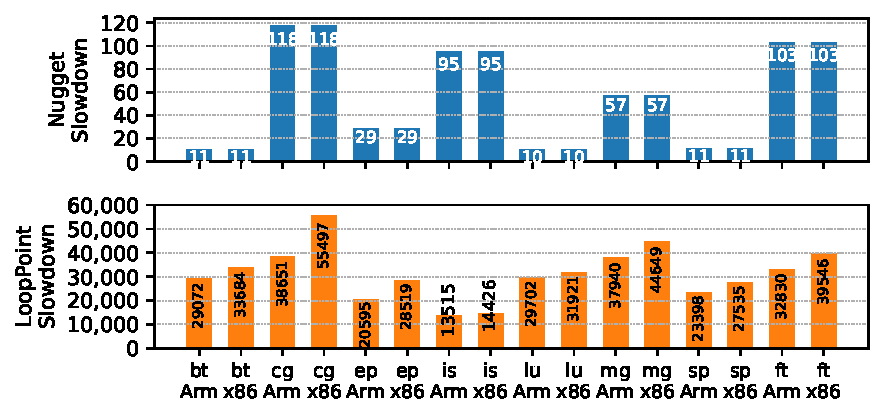
\includegraphics[width=\linewidth]{images/simulation_interval_analysis_overhead_separated.pdf}
    \caption{Interval analysis overhead via Nugget and functional simulation.}
    \label{fig:simulation_interval_analysis_overhead}
\end{figure}

As shown in Figure~\ref{fig:simulation_interval_analysis_overhead}, we observe an average $577.65\times$ reduction in interval analysis overhead when using Nugget instead of gem5's functional simulation.
The overhead on the order of tens of thousands in functional simulation highlights its impracticality for interval analysis in large applications.
On average, Nugget incurs a slowdown of $54\times$, with a maximum of $118\times$ for the ``cg'' benchmark.
By comparison, LoopPoint's average overhead is $31,\!343\times$, peaking at $55,\!497\times$ for ``cg-x86.''

Overall, multi-threaded workloads amplify interval analysis overhead because their baseline execution times are significantly \revision{shorter (due to parallelism) while} the analysis itself incurs greater cost from synchronization requirements.
The single-threaded workloads in Figure~\ref{fig:interval_analysis_overhead} exhibit much lower overheads, which we discuss further in Section~\ref{sec:mix_of_workload_types}.
The ``cg'' benchmark has the shortest execution time in this experiment (0.28 seconds), which further amplifies the measured overhead for both methods.
The ``is'' benchmark exhibits the lowest overhead under functional simulation but still incurs a $95\times$ slowdown with Nugget, primarily due to the frequent executions of interval analysis hooks, as discussed in Section~\ref{sec:hook_overhead}.
The ``mg'' and ``ft'' benchmarks show relatively high overhead for both methods because their parallel regions increase synchronization costs during interval analysis, which in turn adds further simulation overhead.
We examine the relationship between synchronization and overhead in more detail in Section~\ref{sec:scaling_with_number_of_threads}.

In addition to its lower overhead, Nugget offers a key practical advantage: it requires only a single interval analysis run to generate nuggets that can be executed across multiple architectures.
In contrast, LoopPoint must repeat interval analysis for every binary variant or target architecture, significantly increasing its total cost.

\subsubsection{Mix of Workload Types}
\label{sec:mix_of_workload_types}

\begin{figure}[!t]
    \centering
    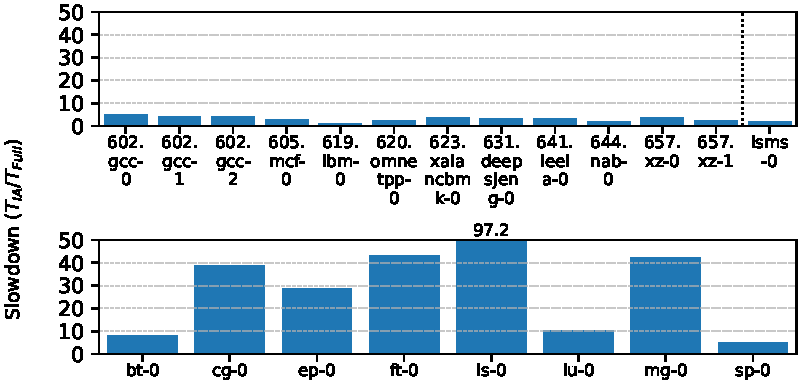
\includegraphics[width=\linewidth]{images/interval_analysis_overhead_2panel.pdf}
    \caption{Interval analysis overhead via Nugget across different workloads.}
    \label{fig:interval_analysis_overhead}
\end{figure}

We also evaluate overhead across a mix of workload types.
For single-threaded workloads, we use the SPEC~CPU2017 suite with the \texttt{ref} input size and the LSMS benchmark with the \texttt{Fe} input size.
For multi-threaded workloads, we use the NPB suite with Class ``C'' in this experiment.

Figure~\ref{fig:interval_analysis_overhead} shows the interval analysis slowdown across the evaluated workloads and demonstrates that \textbf{the overhead varies significantly depending on the level of synchronization}.
The average observed overhead is \(3\times\) for SPEC~CPU2017, \(2\times\) for LSMS, and \(34\times\) for NPB.
The overhead remains low for SPEC~CPU2017 and LSMS because they are single-threaded workloads, which simplifies interval analysis by eliminating the need for synchronization.
In contrast, the high overhead for NPB arises from the synchronization required during multi-threaded interval analysis, particularly due to aggregation across threads.
As synchronization demands increase, so does the overhead, a relationship we explore further in Section~\ref{sec:scaling_with_number_of_threads}.

\textbf{To demonstrate the flexibility of our approach across host machines, we repeat the interval analysis on two distinct systems listed in Table~\ref{tab:system-configuration} and find consistent results across both platforms for single-threaded workloads, with one corner case.}
For SPEC~CPU2017, interval analysis results are identical across the two systems.
For NPB, the multi-threaded nature of the benchmarks introduces variability between runs (even on the same host), a well-known challenge in multi-threaded sampling that is beyond the scope of this work~\cite{looppoint,barrier_point}.
For LSMS, we observe minor differences in the execution frequency of some IRBBs, which we attribute to differences in floating-point precision across CPUs.
In particular, the number of iterations in certain data-driven loops in LSMS is influenced by the underlying architecture's precision.
Such differences could affect nugget representativeness if a marker IRBB is sensitive to these variations.
Nevertheless, as shown in Section~\ref{sec:sample_validation}, nuggets generated from interval analysis on one system still achieve low prediction error when validated on the other system for LSMS.

\subsubsection{Scaling with Number of Threads}
\label{sec:scaling_with_number_of_threads}

\begin{figure}[!t]
    \centering
    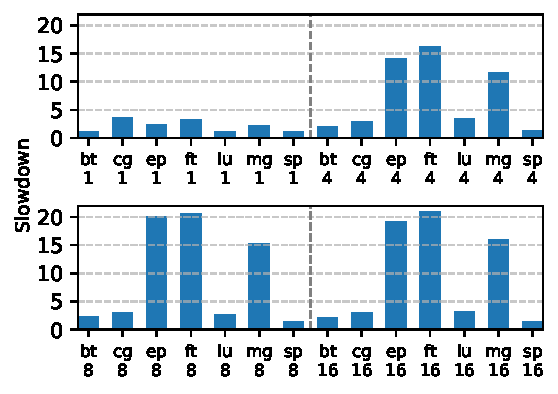
\includegraphics[width=\linewidth]{images/class_d_overhead_analysis_2panel.pdf}
    \caption{Interval analysis overhead via Nugget across different numbers of threads.}
    \label{fig:class_d_overhead_analysis}
\end{figure}

Finally, we study how interval analysis overhead scales with the number of threads.
For this experiment, we use the NPB suite with Class ``D'' inputs and vary the thread count across \{1, 4, 8, 16\}.
To ensure fair comparisons, all overheads are normalized to the execution time of the original workload running with a single thread.

As shown in Figure~\ref{fig:class_d_overhead_analysis}, most workloads exhibit increasing overhead with higher thread counts, consistent with our expectation that more threads lead to greater synchronization overhead.
However, this growth is not uniform across all workloads because not all of them require the same level of synchronization during interval analysis, as not all hooks are executed within parallel regions.
For ``bt'', ``cg'', ``lu'', and ``sp'', the consistently low slowdown as the thread count increases suggests that hooks are not frequently executed within parallel regions for these benchmarks.
In contrast, ``mg'' and ``ft'' show a significant increase in overhead with more threads, indicating that these benchmarks require more synchronization during interval analysis---likely due to the complexity of their parallel regions.

Even at higher thread counts (up to $16\times$), Nugget maintains overheads that are orders of magnitude lower than those of functional simulation-based interval analysis (Figure~\ref{fig:simulation_interval_analysis_overhead}).

\subsubsection{Summary}\label{sec:interval_analysis_overhead_summary}

Our experiments show that Nugget achieves orders-of-magnitude lower interval analysis overhead compared to functional simulation, with an average reduction of over $577.65\times$ relative to LoopPoint for multi-threaded workloads.
It also produces consistent analysis results across different host machines, demonstrating its portability.

By enabling fast, binary-independent interval analysis, even for large workloads, Nugget successfully meets Goal~1.

In the following sections, we build upon this foundation to demonstrate how Nugget supports a variety of sampling methodologies (Goal~2) and enables rapid validation of selected samples on real hardware (Goal~3), further establishing its effectiveness for sampling methodology research.
